%%%%%%%%%%%%%%%%%%%%%%% file template.tex %%%%%%%%%%%%%%%%%%%%%%%%%
%
% This is a general template file for the LaTeX package SVJour3
% for Springer journals.          Springer Heidelberg 2010/09/16
%
% Copy it to a new file with a new name and use it as the basis
% for your article. Delete % signs as needed.
%
% This template includes a few options for different layouts and
% content for various journals. Please consult a previous issue of
% your journal as needed.
%
%%%%%%%%%%%%%%%%%%%%%%%%%%%%%%%%%%%%%%%%%%%%%%%%%%%%%%%%%%%%%%%%%%%
%
% First comes an example EPS file -- just ignore it and
% proceed on the \documentclass line
% your LaTeX will extract the file if required
\begin{filecontents*}{example.eps}
    %!PS-Adobe-3.0 EPSF-3.0
    %%BoundingBox: 19 19 221 221
    %%CreationDate: Mon Sep 29 1997
    %%Creator: programmed by hand (JK)
    %%EndComments
    gsave
    newpath
    20 20 moveto
    20 220 lineto
    220 220 lineto
    220 20 lineto
    closepath
    2 setlinewidth
    gsave
    .4 setgray fill
    grestore
    stroke
    grestore
\end{filecontents*}
%
\RequirePackage{fix-cm}
%
%\documentclass{svjour3}                     % onecolumn (standard format)
%\documentclass[smallcondensed]{svjour3}     % onecolumn (ditto)
\documentclass[smallextended]{svjour3}       % onecolumn (second format)
%\documentclass[twocolumn]{svjour3}          % twocolumn
%
\smartqed  % flush right qed marks, e.g. at end of proof
%
\usepackage{graphicx}
%
% \usepackage{mathptmx}      % use Times fonts if available on your TeX system
%
% insert here the call for the packages your document requires
%\usepackage{latexsym}
% etc.
%
% please place your own definitions here and don't use \def but
% \newcommand{}{}
%
% Insert the name of "your journal" with
% \journalname{myjournal}
%
\begin{document}

    \title{Neural Networks and their Application in Reinforcement Learning%\thanks{Grants or other notes
    %about the article that should go on the front page should be
    %placed here. General acknowledgments should be placed at the end of the article.}
    }
    \subtitle{Reinforcement Learning Seminar -- Winter Semester 2018/19}

    %\titlerunning{Short form of title}        % if too long for running head

    \author{Fabian Otto
    %    \and Second Author %etc.
    }

    %\authorrunning{Short form of author list} % if too long for running head

    \institute{Fabian Otto \at
    Technische Universit\"at Darmstadt, Computer Science Department\\
    %    Tel.: +123-45-678910\\
    %    Fax: +123-45-678910\\
    \email{fabian.otto@stud.tu-darmstadt.de}           %  \\
    %             \emph{Present address:} of F. Author  %  if needed
    %    \and
    %    S. Author \at
    %    second address
    }

    \date{Received: date / Accepted: date}
    % The correct dates will be entered by the editor


    \maketitle

    \begin{abstract}
        Insert your abstract here. Include keywords, PACS and mathematical
        subject classification numbers as needed.
        \keywords{Reinforcement Learning\and Neural Networks}
        % \PACS{PACS code1 \and PACS code2 \and more}
        % \subclass{MSC code1 \and MSC code2 \and more}
    \end{abstract}

    \section{Introduction}
    \label{sec:intro}
    Give introduction with NN hype or similar things. As well as the importance.
    Define RL and the method in general.
    Show clear distinction to SL.
    \section{Definition of Neural Networks}
    \label{sec:def}
    \cite{RefB} and \cite{RefJ}.
    Describe formally how NN are working, how can they be trained, what other methods do we have, etc.
    \section{History of Neural Networks}
    \label{sec:history}
    (see Sect.~\ref{sec:1}).
    What did lead to the rise and fall of NNs throughout time.
    Create good transition to recent approaches.

    \section{Recent Approaches in Reinforcement Learning}
    \label{sec:recent}
    \subsection{Algorithms}
    \label{sec:algo}
    \subsection{Application Areas}
    \label{sec:games}
    Talk about DeepMinds AlphaZero, TDGammon, Atari Game Systems, e.g. Minh
    But also applications outside of Games, maybe seperate this into two different subsections.
    \paragraph{Paragraph headings}
    \begin{equation}
        a^2+b^2=c^2
    \end{equation}

    % For one-column wide figures use
    \begin{figure}
        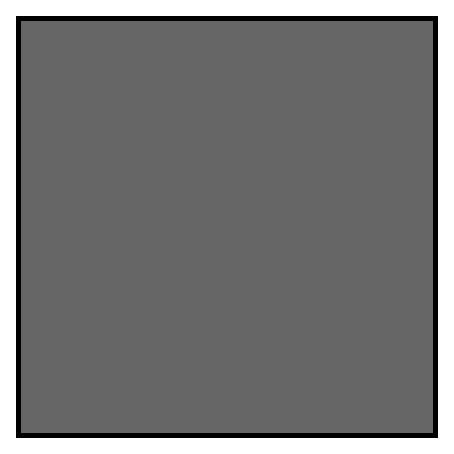
\includegraphics{example.eps}
        % figure caption is below the figure
        \caption{Please write your figure caption here}
        \label{fig:1}
    \end{figure}
    %
    % For two-column wide figures use
    \begin{figure*}
        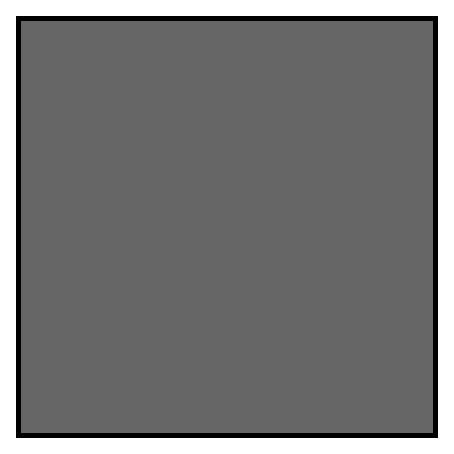
\includegraphics[width=0.75\textwidth]{example.eps}
        % figure caption is below the figure
        \caption{Please write your figure caption here}
        \label{fig:2}
    \end{figure*}

    \begin{table}
        % table caption is above the table
        \caption{Please write your table caption here}
        \label{tab:1}
        \begin{tabular}{lll}
            \hline\noalign{\smallskip}
            first & second & third  \\
            \noalign{\smallskip}\hline\noalign{\smallskip}
            number & number & number \\
            number & number & number \\
            \noalign{\smallskip}\hline
        \end{tabular}
    \end{table}


    %\begin{acknowledgements}
    %If you'd like to thank anyone, place your comments here
    %and remove the percent signs.
    %\end{acknowledgements}

    % BibTeX users please use one of
    %\bibliographystyle{spbasic}      % basic style, author-year citations
    \bibliographystyle{spmpsci}      % mathematics and physical sciences
    %\bibliographystyle{spphys}       % APS-like style for physics
    \bibliography{resources.bib}
    % name your BibTeX data base

\end{document}

